\begin{theo}[Vector]{Vector}
    Een \textbf{Vector} is een grootheid met een grootte, net zoals een scalar, een richting en een zin.
    \begin{itemize}
        \item \textbf{Eenheidsvector:} een vector, meestal genoteerd als $ \hat{u} $ waarvan de lengte 1 is
        \item \textbf{Plaatsvector:} vector van een punt ten opzicht van het coördinatenstelsel
        \item \textbf{Relatieve positievector:} vector tussen twee punten
    \end{itemize}
\end{theo}

\begin{pro}[Eigenschappen van vectoren]{Eigenschappen van vectoren}
    Elke vector kan je zien als een som van meerdere vectoren, namelijk zijn coördinaatvectoren. We verklaren tweedimensionaal:
    
    \begin{equation*}
        \Vec{r} = r_x\hat{i} + r_y\hat{j}
    \end{equation*}

    \noindent Nu we dit weten kunen we som en verschil van twee vectoren gewoon zien als het optellen of aftrekken van de coördinaten. Deze coördinaten of vectorcomponenten kunnen we makkelijk berekenen, namelijk: 

    \begin{equation*}
        r_x = r\cos(\theta),\ r_y = r\sin(\theta)
    \end{equation*}
    
    \begin{center}
        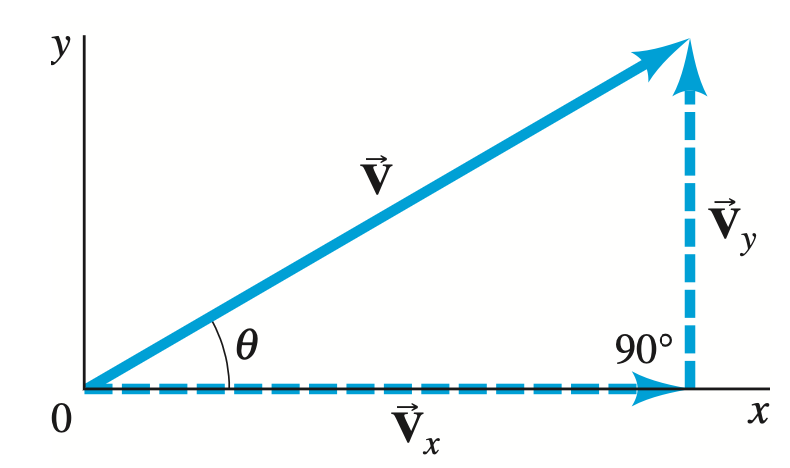
\includegraphics[scale = 0.4]{Images/Inleiding/Vectorcomponenten.png}
        \\
        ($\Vec{r} = \Vec{V}$ op de tekening)
    \end{center}
    
    \noindent Hieruit kunnen we het volgende afleiden:
    
    \begin{equation*}
        r = |r| = \sqrt{r_x^2 + r_y^2}, \ \theta = \tan^{-1}\dfrac{r_y}{r_x}
    \end{equation*}

    \noindent Deze samenvatting zal vaak gebruik maken van de volgende notatie met $\hat{u}$ een eenheidsvector met dezelfde richting als $\Vec{r}$:

    \begin{equation*}
        \Vec{r} = |r|\hat{u}
    \end{equation*}

    \noindent Dit volgt uit het feit dat 
    
    \begin{equation*}
        \hat{u} = \dfrac{\Vec{r}}{|r|}
    \end{equation*}
\end{pro}

\newpage

\begin{theo}[Dot product]{Dot product}
    Het dot product kan meetkundig geïnterpreteerd worden als de grootte van een vector maal de projectie van de andere vector. De formule is:
    \begin{equation*}
        \Vec{A} \cdot \Vec{B} = \sum_{i=1}^n a_ib_i = AB\cos{\theta}
    \end{equation*}
    \vspace{-0.5cm}
\end{theo}

\begin{pro}[Eigenschappen van het dot product]{pro - Dot product}
    \begin{itemize} 
    \item commutatief: $ A \cdot B = B \cdot A $
    \item distributief t.o.v. de optelling: $ A \cdot (B+C) = A \cdot B + A \cdot C $
\end{itemize}
\end{pro}

\begin{theo}[Vector product]{Vector product}
    De formule van het vector product geeft als uitkomst geen scalar, maar een gloednieuwe vector loodrecht op A en B . Hier deze formule:
    \begin{equation*}
        \Vec{A} \times \Vec{B} = \begin{vmatrix}
         \hat{i} & \hat{j} & \hat{k}\\ 
         A_x & A_y & A_z\\
         B_x & B_y & B_z  \end{vmatrix} = AB\sin(\theta) \hat{u}
    \end{equation*}
    met $\hat{u}$ een gerichte eenheidsvector loodrecht op het vlak.
\end{theo}

\begin{pro}[Eigenschappen van het vector product]{pro - Vector product}
    \begin{itemize} 
        \item \textbf{niet} commutatief: $ A \times B = \textbf{-}B \times A $
        \item distributief t.o.v. de optelling: $ A \times (B+C) = A \times B + A \times C $
    \end{itemize}
\end{pro}
